% Figure 5.11: Mentor Matching Pipeline
% Compile with: pdflatex fig_5_11_mentor_pipeline.tex

\documentclass[border=10pt]{standalone}
\usepackage{tikz}
\usetikzlibrary{shapes.geometric, arrows.meta, positioning}
\usepackage{xcolor}

% Professional academic color palette
\definecolor{embedblue}{RGB}{176, 196, 222}    % Light steel blue
\definecolor{layer1}{RGB}{70, 130, 180}        % Steel blue
\definecolor{denseorange}{RGB}{222, 184, 135}  % Burlywood
\definecolor{outputpurple}{RGB}{186, 175, 201} % Lavender gray
\definecolor{accentteal}{RGB}{119, 176, 166}   % Muted teal
\definecolor{inputgray}{RGB}{220, 220, 220}
\definecolor{textdark}{RGB}{33, 33, 33}

\begin{document}
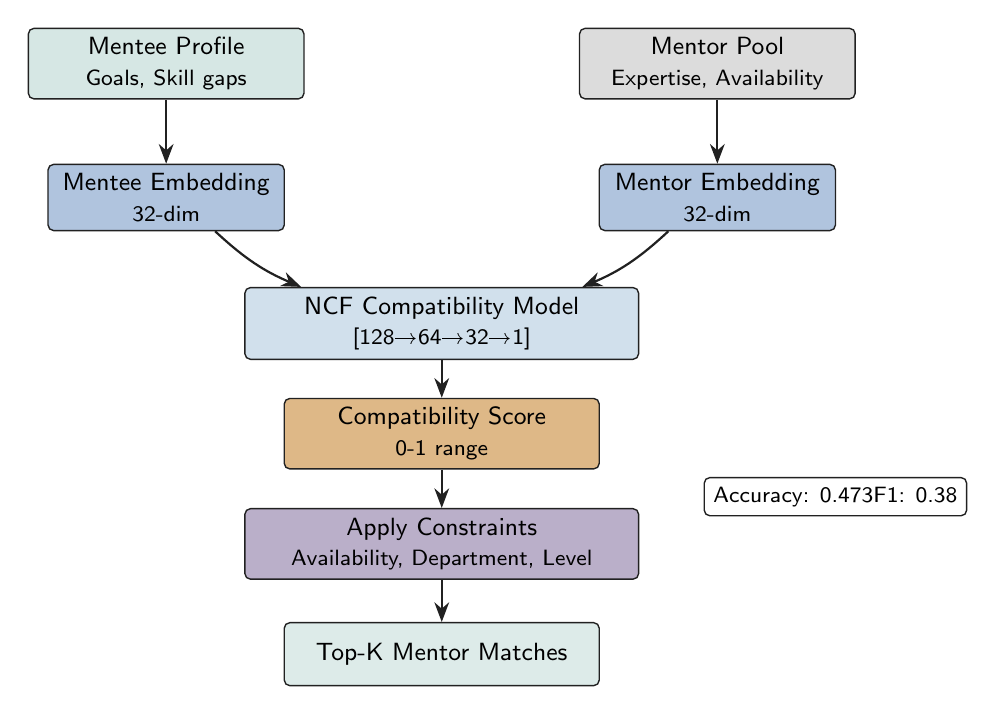
\begin{tikzpicture}[
    node distance=1cm,
    layer/.style={rectangle, draw=textdark, rounded corners=2pt, minimum width=3cm, minimum height=0.8cm, align=center, font=\small\sffamily, line width=0.5pt},
    arrow/.style={-{Stealth[length=2.5mm]}, thick, color=textdark},
]

% Inputs
\node[layer, fill=accentteal!30, minimum width=3.5cm] (mentee) at (-3.5, 5.5) {Mentee Profile\\{\footnotesize\sffamily Goals, Skill gaps}};
\node[layer, fill=inputgray, minimum width=3.5cm] (mentor) at (3.5, 5.5) {Mentor Pool\\{\footnotesize\sffamily Expertise, Availability}};

% Embeddings
\node[layer, fill=embedblue] (menteemb) at (-3.5, 3.8) {Mentee Embedding\\{\footnotesize\sffamily 32-dim}};
\node[layer, fill=embedblue] (mentoremb) at (3.5, 3.8) {Mentor Embedding\\{\footnotesize\sffamily 32-dim}};

\draw[arrow] (mentee) -- (menteemb);
\draw[arrow] (mentor) -- (mentoremb);

% NCF
\node[layer, fill=layer1!25, minimum width=5cm] (ncf) at (0, 2.2) {NCF Compatibility Model\\{\footnotesize\sffamily [128→64→32→1]}};

\draw[arrow] (menteemb) to[bend right=10] (ncf);
\draw[arrow] (mentoremb) to[bend left=10] (ncf);

% Scoring
\node[layer, fill=denseorange, minimum width=4cm] (score) at (0, 0.8) {Compatibility Score\\{\footnotesize\sffamily 0-1 range}};

\draw[arrow] (ncf) -- (score);

% Constraints
\node[layer, fill=outputpurple, minimum width=5cm] (constraints) at (0, -0.6) {Apply Constraints\\{\footnotesize\sffamily Availability, Department, Level}};

\draw[arrow] (score) -- (constraints);

% Output
\node[layer, fill=accentteal!25, minimum width=4cm] (output) at (0, -2) {Top-K Mentor Matches};

\draw[arrow] (constraints) -- (output);

% Metrics
\node[rectangle, draw=textdark, fill=white, rounded corners=2pt, font=\footnotesize\sffamily, line width=0.5pt] at (5, 0) {Accuracy: 0.473\\F1: 0.38};

\end{tikzpicture}
\end{document}
